\documentclass{article}

\usepackage{pgfplots}

\pgfplotsset{compat=1.11}

\begin{document}

%\tracingcommands=2\tracingmacros=2
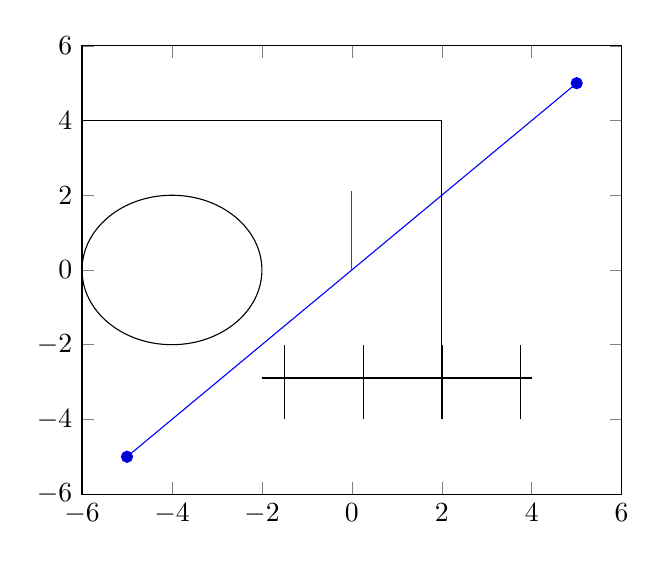
\begin{tikzpicture}
	\begin{axis}
	\addplot+[samples=2] {x};	

	\draw (-6,4) -| (2,-4);

	\draw (-4,0) circle[radius=2];

	% grid with units fails (affine linear map) :-(
	\draw (-2,-4) grid[step=1cm] (4,-2);

	\draw[red] (0,0cm) -- (0,1cm);
	\end{axis}
\end{tikzpicture}

\tikz\draw[red] (0pt,0pt) -- (0pt,1cm);

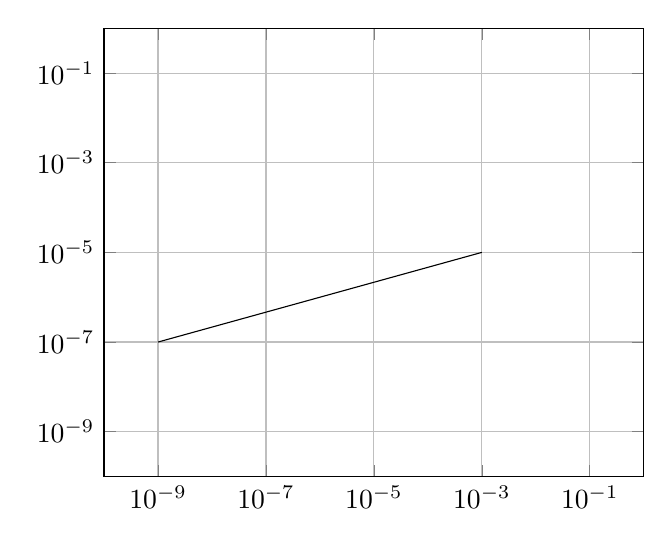
\begin{tikzpicture}
	\begin{loglogaxis}[xmin=1e-10,xmax=1,
		ymin=1e-10,ymax=1,grid=major]

	\draw (1e-9,1e-7) -- (1e-3,1e-5);

	\end{loglogaxis}
\end{tikzpicture}

\begin{tikzpicture}
	\begin{axis}
	\addplot+[samples=2,domain=-5e5:5e5] {x};	

	\draw (-4e5,0) circle[radius=2e5];
	\draw (-6e5,4e5) -| (2e5,-4e5);

	\draw (-2e5,-4e5) grid[step=1cm] (4e5,-2e5);
	\end{axis}
\end{tikzpicture}
\end{document}

